\chapter{示例}{Examples}
\section{用PGF画图}{Draw with PGF}
PGF\citep{tantau:pgf}是非常强大的\LaTeX{}画图宏包,必须承认本人较有洁癖,
加上做的课题没有实验截图,所以整篇论文中的图都是用PGF画的矢量图形。下面主要给出一些论文中
用PGF画图的示例,希望对使用者有所帮助。PGF详细具体的说明请查阅PGF自带的手册,做完里面的Tutorial后,
以各位的高智商应该可以轻松运用了。

当然阁下可以选择方便地插入位图,具体的步骤网上一抓无数,这里就不重复劳动了。

图\ref{fig:mexican_hat}是用PGF+GNUPlot画出墨西哥小波函数的例子。注意,plot file命令中的“/”
是Linux下的路径分隔符,如果你是在Windows下的话需要改为“\textbackslash ”才可以的哦。
\small{
\begin{verbatim}
\begin{figure}[htpb]
    \begin{center}
        \begin{tikzpicture}[>=stealth,thick]
            \draw [->] (-5.5,0) -- (6,0);
            \draw [->] (0, -2.5) -- (0, 5);
            \draw [color=blue] plot file {figures/gnuplot/mexican.table};
            \draw node at (0,0) [below left, color=gray] {$O$};
            \foreach \x in {-5,-4,-3,-2,-1, 1, 2, 3, 4, 5}
                \draw (\x, 1pt) -- (\x, -1pt) node [below=2pt,color=gray] {$\x$};
        \node at (6,0) [below=4pt, color=gray] {$x$};
            \foreach \y/\yy in {-2/-0.2, -1/-0.1, 1/0.1, 2/0.2, 3/0.3, 4/0.4}
                \draw (-1pt, \y) -- (1pt, \y) node [left=6pt,color=gray] {$\yy$};
        \node at (0,5) [left=6pt, color=gray] {$y$};
        \end{tikzpicture}
    \end{center}
    \caption{Mexican Hat Wavelet}
    \label{fig:mexican_hat}
\end{figure}
\end{verbatim}
}

\begin{figure}[htpb]
    \begin{center}
        \begin{tikzpicture}[>=stealth,thick]
            \draw [->] (-5.5,0) -- (6,0);
            \draw [->] (0, -2.5) -- (0, 5);
            \draw [color=blue] plot file {figures/gnuplot/mexican.table};
            \draw node at (0,0) [below left, color=gray] {$O$};
            \foreach \x in {-5,-4,-3,-2,-1, 1, 2, 3, 4, 5}
                \draw (\x, 1pt) -- (\x, -1pt) node [below=2pt,color=gray] {$\x$};
	    \node at (6,0) [below=4pt, color=gray] {$x$};
            \foreach \y/\yy in {-2/-0.2, -1/-0.1, 1/0.1, 2/0.2, 3/0.3, 4/0.4}
                \draw (-1pt, \y) -- (1pt, \y) node [left=6pt,color=gray] {$\yy$};
	    \node at (0,5) [left=6pt, color=gray] {$y$};
        \end{tikzpicture}
    \end{center}
    \caption{Mexican Hat Wavelet}
    \label{fig:mexican_hat}
\end{figure}

当然,我们往往需要画出一些数据处理的示意图,如图\ref{fig:dwt_idwt},就是小波分解和合成的简要示意。
\small{
\begin{verbatim}
\begin{figure}[htpb]
    \begin{center}
        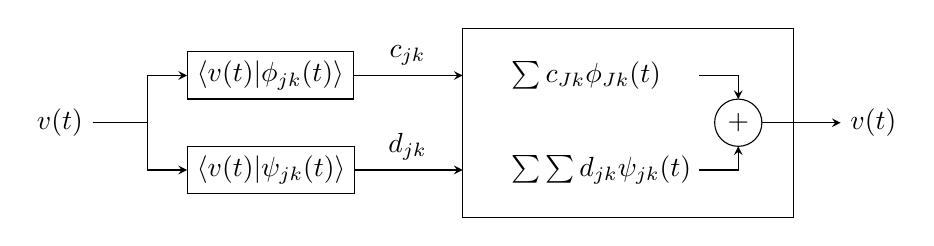
\begin{tikzpicture}[>=stealth]
            \draw [->] (0.3,0) -- (1,0) -- (1,0.6) -- (1.5,0.6);
            \draw node at (0.3,0) [left] {$v(t)$};
            \draw [->] (1.5,0.6) -- (5, 0.6);
            \draw node at (4.3, 0.6) [above] {$c_{jk}$};
            \draw [->] (1,0) -- (1,-0.6) -- (1.5,-0.6);
            \draw [->] (1.5,-0.6) -- (5,-0.6);
            \draw node at (4.3, -0.6) [above] {$d_{jk}$};
            \draw node at (1.5,0.6) [right,rectangle,draw,fill=white] {$\langle
            v(t) | \phi_{jk}(t)\rangle$};
            \draw node at (1.5,-0.6) [right,rectangle,draw,fill=white] {$\langle
            v(t) | \psi_{jk}(t)\rangle$};
            \draw (5,-1.2) rectangle ++ (4.2, 2.4);
            \draw node at (5.5, 0.6) [right] {$\sum c_{Jk}\phi_{Jk}(t)$};
            \draw node at (5.5, -0.6) [right] {$\sum\sum d_{jk}\psi_{jk}(t)$};
            \draw [->] (8,0.6) -- (8.5,0.6) -- ++(0,-0.3);
            \draw [->] (8,-0.6) -- (8.5,-0.6) -- ++(0,0.3);
            \draw (8.5,0) circle (0.3) node {+};
            \draw [->](8.8,0) -- (9.8,0) node [right] {$v(t)$};
        \end{tikzpicture}
    \end{center}
    \caption{离散小波分解与小波合成}
    \label{fig:dwt_idwt}
\end{figure}
\end{verbatim}
}
\begin{figure}[htpb]
    \begin{center}
        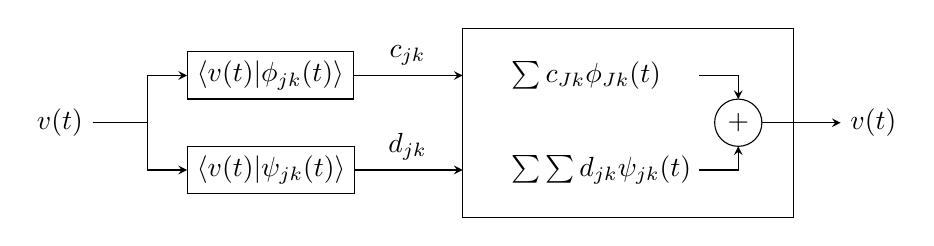
\begin{tikzpicture}[>=stealth]
            \draw [->] (0.3,0) -- (1,0) -- (1,0.6) -- (1.5,0.6);
            \draw node at (0.3,0) [left] {$v(t)$};
            \draw [->] (1.5,0.6) -- (5, 0.6);
            \draw node at (4.3, 0.6) [above] {$c_{jk}$};
            \draw [->] (1,0) -- (1,-0.6) -- (1.5,-0.6);
            \draw [->] (1.5,-0.6) -- (5,-0.6);
            \draw node at (4.3, -0.6) [above] {$d_{jk}$};
            \draw node at (1.5,0.6) [right,rectangle,draw,fill=white] {$\langle
            v(t) | \phi_{jk}(t)\rangle$};
            \draw node at (1.5,-0.6) [right,rectangle,draw,fill=white] {$\langle
            v(t) | \psi_{jk}(t)\rangle$};
            \draw (5,-1.2) rectangle ++ (4.2, 2.4);
            \draw node at (5.5, 0.6) [right] {$\sum c_{Jk}\phi_{Jk}(t)$};
            \draw node at (5.5, -0.6) [right] {$\sum\sum d_{jk}\psi_{jk}(t)$};
            \draw [->] (8,0.6) -- (8.5,0.6) -- ++(0,-0.3);
            \draw [->] (8,-0.6) -- (8.5,-0.6) -- ++(0,0.3);
            \draw (8.5,0) circle (0.3) node {+};
            \draw [->](8.8,0) -- (9.8,0) node [right] {$v(t)$};
        \end{tikzpicture}
    \end{center}
    \caption{离散小波分解与小波合成}
    \label{fig:dwt_idwt}
\end{figure}

图\ref{fig:mra}是简单流程图的示意。
\small{
\begin{verbatim}
\begin{figure}[htpb]
    \begin{center}
        \begin{tikzpicture}[->,node distance=7mm and 5mm,>=stealth,
            mn/.style={
            rectangle,
            draw=white
            }]
            \node (LR) {$L^2(R)$};
            \node (VJ) [right=of LR]{$V_J$};
            \node (VJm1) [right=of VJ] {$V_{J-1}$};
            \node (WJm1) [below=of VJm1] {$W_{J-1}$};
            \node (dots) [right=of VJm1] {$\cdots$};
            \node (V1) [right=of dots] {$V_1$};
            \node (W1) [below=of V1] {$W_1$};
            \node (V0) [right=of V1] {$V_0$};
            \node (W0) [below=of V0] {$W_0$};
            \path (LR) edge (VJ)
            (VJ) edge (VJm1)
            (VJ) edge[in=150,out=330]  (WJm1)
            (VJm1) edge (dots)
            (dots) edge (V1)
            (dots) edge[in=150,out=330] (W1)
            (V1) edge (V0)
            (V1) edge [in=150,out=330] (W0)
            ;
        \end{tikzpicture}
    \end{center}
    \caption{多分辨分析示意图}
    \label{fig:mra}
\end{figure}
\end{verbatim}
}

\begin{figure}[htpb]
    \begin{center}
        \begin{tikzpicture}[->,node distance=7mm and 5mm,>=stealth,
            mn/.style={
            rectangle,
            draw=white
            }]
            \node (LR) {$L^2(R)$};
            \node (VJ) [right=of LR]{$V_J$};
            \node (VJm1) [right=of VJ] {$V_{J-1}$};
            \node (WJm1) [below=of VJm1] {$W_{J-1}$};
            \node (dots) [right=of VJm1] {$\cdots$};
            \node (V1) [right=of dots] {$V_1$};
            \node (W1) [below=of V1] {$W_1$};
            \node (V0) [right=of V1] {$V_0$};
            \node (W0) [below=of V0] {$W_0$};
            \path (LR) edge (VJ)
            (VJ) edge (VJm1)
            (VJ) edge[in=150,out=330]  (WJm1)
            (VJm1) edge (dots)
            (dots) edge (V1)
            (dots) edge[in=150,out=330] (W1)
            (V1) edge (V0)
            (V1) edge [in=150,out=330] (W0)
            ;
        \end{tikzpicture}
    \end{center}
    \caption{多分辨分析示意图}
    \label{fig:mra}
\end{figure}


图\ref{fig:mallat}所示是复杂一些的流程图。
\small{
\begin{verbatim}
\begin{figure}[htpb]
    \begin{center}
        \begin{tikzpicture}[node distance=5mm and 12mm,>=stealth,
            an/.style={
            rectangle,
            draw=black
            },
            pn/.style={coordinate},
            cn/.style={
            font=\small
            }
            ]
            \node (Vt) [an] {$V(t)$};
            \node (C2) [an, above right=of Vt]{$C_2$};
            \node (D2) [an, below right=of Vt]{$D_2$};
            \node (C1) [an, above right=of C2]{$C_1$};
            \node (D1) [an, below right=of C2]{$D_1$};
            \node (C0) [an, above right=of C1]{$C_0$};
            \node (D0) [an, below right=of C1]{$D_0$};
            \node (C1') [an, below right=of C0]{$C_1'$};
            \node (C2') [an, below right=of C1']{$C_2'$};
            \node (pC1') [pn,right=of D1,xshift=24mm] {};
            \node (VT') [an, below right=of C2']{$V(t)'$};
            \node (pC2') [pn,right=of D2,xshift=60mm] {};
            \path
                (Vt) edge [->,out=10, in=190] node[cn,left,pos=0.8] {$H, \downarrow2\,$} (C2)
                (Vt) edge [->,out=-10, in=-190] node[cn,left,pos=0.8] {$G, \downarrow2\,$} (D2)
                (C2) edge [->,out=10, in=190] node[cn,left,pos=0.8] {$H, \downarrow2\,$} (C1)
                (C2) edge [->,out=-10, in=-190] node[cn,left,pos=0.8] {$G, \downarrow2\,$} (D1)
                (C1) edge [->,out=10, in=190] node[cn,left,pos=0.8] {$H, \downarrow2\,$} (C0)
                (C1) edge [->,out=-10, in=-190] node[cn,left,pos=0.8] {$G, \downarrow2\,$} (D0)
                (C0) edge  [->,out=-10, in=-190] node[cn,right,pos=0.2] {$\,\uparrow2,H^*$} (C1')
                (D0) edge [->,out=0,in=190] node[cn,right,pos=0.2] {$\,\uparrow2,G^*$} (C1')
                (C1') edge  [->,out=-10, in=-190] node[cn,right,pos=0.2] {$\,\uparrow2,H^*$} (C2')
                (D1) edge node[cn,above,pos=0.6] {$\,\uparrow2,G^*$}(pC1')
                (pC1') edge [->,out=0,in=200]  (C2')
                (C2') edge  [->,out=-10, in=-190] node[cn,right,pos=0.2] {$\,\uparrow2,H^*$} (VT')
                (D2) edge node[cn,above,pos=0.57] {$\,\uparrow2,G^*$} (pC2')
                (pC2') edge [->,out=0,in=190] (VT')
            ;
        \end{tikzpicture}
    \end{center}
    \caption{Mallat塔式算法示意图}
    \label{fig:mallat}
\end{figure}
\end{verbatim}
}
\begin{figure}[htpb]
    \begin{center}
        \begin{tikzpicture}[node distance=5mm and 12mm,>=stealth,
            an/.style={
            rectangle,
            draw=black
            },
            pn/.style={coordinate},
            cn/.style={
            font=\small
            }
            ]
            \node (Vt) [an] {$V(t)$};
            \node (C2) [an, above right=of Vt]{$C_2$};
            \node (D2) [an, below right=of Vt]{$D_2$};
            \node (C1) [an, above right=of C2]{$C_1$};
            \node (D1) [an, below right=of C2]{$D_1$};
            \node (C0) [an, above right=of C1]{$C_0$};
            \node (D0) [an, below right=of C1]{$D_0$};
            \node (C1') [an, below right=of C0]{$C_1'$};
            \node (C2') [an, below right=of C1']{$C_2'$};
            \node (pC1') [pn,right=of D1,xshift=24mm] {};
            \node (VT') [an, below right=of C2']{$V(t)'$};
            \node (pC2') [pn,right=of D2,xshift=60mm] {};
            \path
                (Vt) edge [->,out=10, in=190] node[cn,left,pos=0.8] {$H, \downarrow2\,$} (C2)
                (Vt) edge [->,out=-10, in=-190] node[cn,left,pos=0.8] {$G, \downarrow2\,$} (D2)
                (C2) edge [->,out=10, in=190] node[cn,left,pos=0.8] {$H, \downarrow2\,$} (C1)
                (C2) edge [->,out=-10, in=-190] node[cn,left,pos=0.8] {$G, \downarrow2\,$} (D1)
                (C1) edge [->,out=10, in=190] node[cn,left,pos=0.8] {$H, \downarrow2\,$} (C0)
                (C1) edge [->,out=-10, in=-190] node[cn,left,pos=0.8] {$G, \downarrow2\,$} (D0)
                (C0) edge  [->,out=-10, in=-190] node[cn,right,pos=0.2] {$\,\uparrow2,H^*$} (C1')
                (D0) edge [->,out=0,in=190] node[cn,right,pos=0.2] {$\,\uparrow2,G^*$} (C1')
                (C1') edge  [->,out=-10, in=-190] node[cn,right,pos=0.2] {$\,\uparrow2,H^*$} (C2')
                (D1) edge node[cn,above,pos=0.6] {$\,\uparrow2,G^*$}(pC1')
                (pC1') edge [->,out=0,in=200]  (C2')
                (C2') edge  [->,out=-10, in=-190] node[cn,right,pos=0.2] {$\,\uparrow2,H^*$} (VT')
                (D2) edge node[cn,above,pos=0.57] {$\,\uparrow2,G^*$} (pC2')
                (pC2') edge [->,out=0,in=190] (VT')
            ;
        \end{tikzpicture}
    \end{center}
    \caption{Mallat塔式算法示意图}
    \label{fig:mallat}
\end{figure}

\section{表格}{Tables}
    表格一般可以用tabular、tabularx、longtable等环境,我自己的论文中只用到了longtable,所以下面
    就举个简单的例子。

\begin{longtable}[c]{llll}
    \caption{longtable示例}\\ \hline
        \textsf{项目1}&    \textsf{项目2}&    \textsf{项目3}&    \textsf{项目3}\\ \hline
    \endfirsthead
        \multicolumn{4}{r}{\footnotesize{续上页表\thetable}} \\
        \hline \textsf{项目1}&    \textsf{项目2}&    \textsf{项目3}&    \textsf{项目3}\\ \hline
    \endhead
        \hline \multicolumn{4}{r}{\footnotesize{表格接下页\ldots}}
    \endfoot
        \hline
    \endlastfoot
        拼命打字&    认真画图&    好好写程序&    早睡早起\\
        拼命打字&    认真画图&    好好写程序&    早睡早起\\
        拼命打字&    认真画图&    好好写程序&    早睡早起\\
        拼命打字&    认真画图&    好好写程序&    早睡早起\\
        拼命打字&    认真画图&    好好写程序&    早睡早起\\
        拼命打字&    认真画图&    好好写程序&    早睡早起\\
        拼命打字&    认真画图&    好好写程序&    早睡早起\\
        拼命打字&    认真画图&    好好写程序&    早睡早起\\
        拼命打字&    认真画图&    好好写程序&    早睡早起\\
        拼命打字&    认真画图&    好好写程序&    早睡早起\\
        拼命打字&    认真画图&    好好写程序&    早睡早起\\
        拼命打字&    认真画图&    好好写程序&    早睡早起\\
        拼命打字&    认真画图&    好好写程序&    早睡早起\\
        拼命打字&    认真画图&    好好写程序&    早睡早起\\
        拼命打字&    认真画图&    好好写程序&    早睡早起\\
        拼命打字&    认真画图&    好好写程序&    早睡早起\\
        拼命打字&    认真画图&    好好写程序&    早睡早起\\
        拼命打字&    认真画图&    好好写程序&    早睡早起\\
        拼命打字&    认真画图&    好好写程序&    早睡早起\\
        拼命打字&    认真画图&    好好写程序&    早睡早起\\
        拼命打字&    认真画图&    好好写程序&    早睡早起\\
        拼命打字&    认真画图&    好好写程序&    早睡早起\\
        拼命打字&    认真画图&    好好写程序&    早睡早起\\
        拼命打字&    认真画图&    好好写程序&    早睡早起\\
        拼命打字&    认真画图&    好好写程序&    早睡早起\\
        拼命打字&    认真画图&    好好写程序&    早睡早起\\
        拼命打字&    认真画图&    好好写程序&    早睡早起\\
        拼命打字&    认真画图&    好好写程序&    早睡早起\\
        拼命打字&    认真画图&    好好写程序&    早睡早起\\
        拼命打字&    认真画图&    好好写程序&    早睡早起\\
        拼命打字&    认真画图&    好好写程序&    早睡早起\\
\end{longtable}

\section{参考文献的加入}{Adding Bibliographies}
参考文献可以用Google的学术搜索获得\BibTeX{}的格式\citep{zhujianpin:2009}。首先打开Google的学术搜索,在搜索按钮边上有一个偏好设置的链接。进入后,在页面的最下角有一个Bibliography Manager,选择Show links to import 
into BibTeX。这样当你搜索到你要加入的文献的时候,点 Import to BibTeX就能打开一个已经完成的BibTeX条目了。当然,为了保证整体的英文名子风格统一,你需要检查一下作者英文名字的大小写、缩写是否和要求的一致。
